\documentclass{article}
\usepackage[utf8]{inputenc}
\usepackage[english]{babel}
\usepackage{graphicx}
\usepackage{subcaption}
\usepackage{fancyvrb}
\usepackage{hyperref}

\hypersetup{
    colorlinks=true,
    urlcolor=blue,
}

\title{\textbf{CS550 Advanced Operating Systems\\Programming Assignement 1\\Manual}}
\author{Florentin \textsc{Bekier}\\Rémi \textsc{Blaise}}
\date{}

\begin{document}

\maketitle

\section{Introduction}

This document will guide you through the installation and usage of our project. As detailed in the Design Document, this project contains two different software: \textbf{Index}, located in the \Verb+index+ folder, and \textbf{Peer}, located in the \Verb+peer+ folder. Please follow the following steps for each of the software.

\section{Prerequisite}

Both software are developed using Node.js (version 12.14.1). Therefore, you will need to have it installed on your computer to use them. If you don't have Node.js installed yet, follow the following steps:

\subsection{Mac and Linux users}

First, install \Verb+nvm+ (Node Version Manager) by running the following command in a terminal:

\begin{Verbatim}
curl -o- https://raw.githubusercontent.com/nvm-sh/nvm/v0.35.2/install.sh | bash
\end{Verbatim}

\noindent This command should install \Verb+nvm+ on your machine. Now you need to install the right version of Node.js. Close and reopen your terminal and type this command:

\begin{Verbatim}
nvm install 12
\end{Verbatim}

\noindent Now you should have Node.js installed. You can check that Node.js is running with the right version using this command:

\begin{Verbatim}
node -v
\end{Verbatim}

\begin{figure}
	\centering
	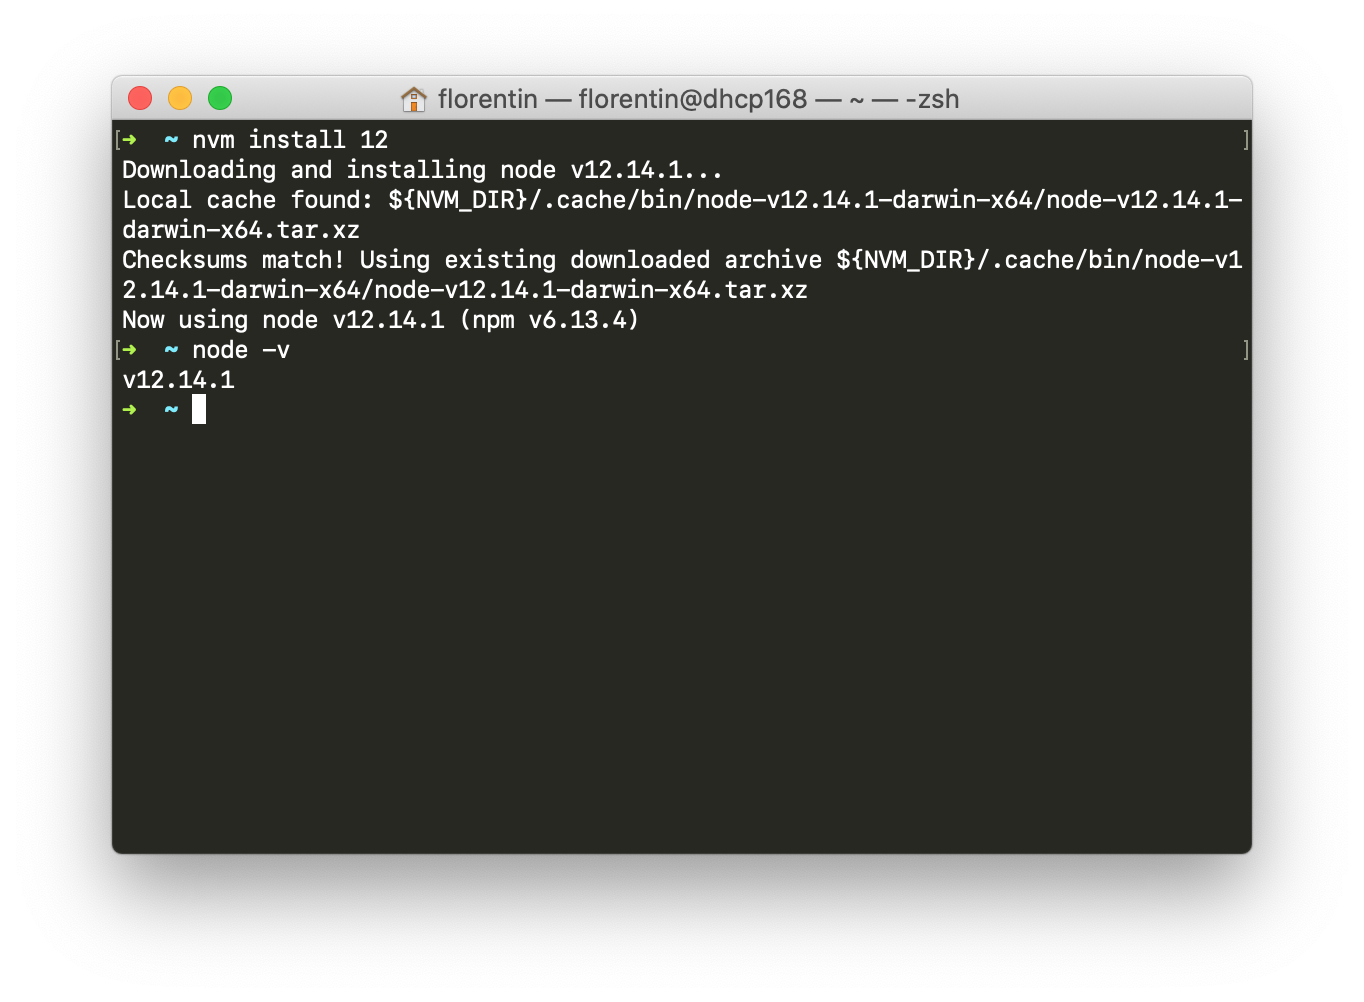
\includegraphics[width=0.7\linewidth]{assets/nvm.png}
	\caption{Node.js installation on macOS}
	\label{fig:nvm}
\end{figure}

\subsection{Windows users}

Download the Node.js Installer for \href{https://nodejs.org/dist/v12.14.1/node-v12.14.1-x86.msi}{32 bits} or \href{https://nodejs.org/dist/v12.14.1/node-v12.14.1-x64.msi}{64 bits} and execute it to install Node.js. \textbf{Make sure to check the box asking to install all the necessary tools}.

\noindent When the installation is finished, open a new Command Prompt window and run the following command to check that Node.js is running with the right version:

\begin{Verbatim}
node -v
\end{Verbatim}

\begin{figure}[h!]
	\centering
	\begin{subfigure}[b]{0.45\linewidth}
		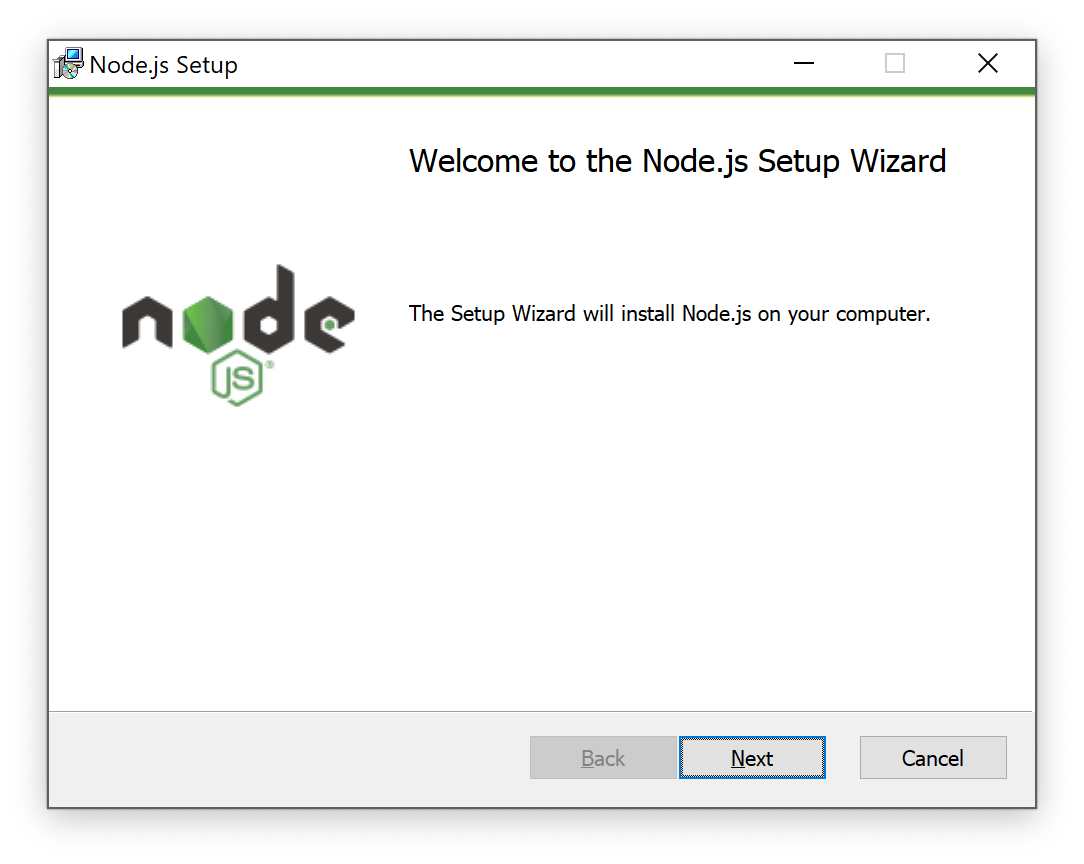
\includegraphics[width=\linewidth]{assets/node-installer-windows.png}
		\caption{Node.js Installer}
	\end{subfigure}
	\begin{subfigure}[b]{0.45\linewidth}
		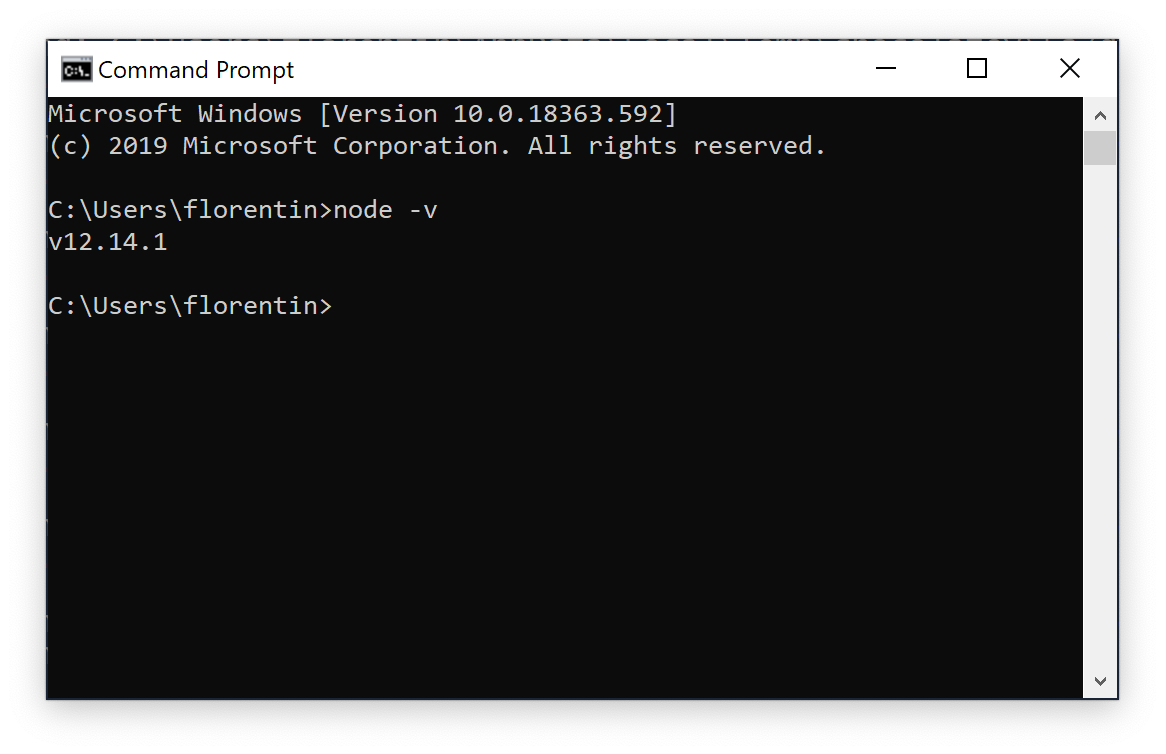
\includegraphics[width=\linewidth]{assets/node-cmd-windows.png}
		\caption{Command Prompt}
	\end{subfigure}
	\caption{Node.js installation on Windows}
	\label{fig:node-windows}
\end{figure}  

\section{Installation}

The installation process is indentical for both the \textbf{Index} and \textbf{Peer} software. First, you should go to the software folder (\Verb+index+ or \Verb+peer+) and open a terminal or a Command Prompt. Then, you will need to install the software dependencies by typing this command:

\begin{Verbatim}
npm install
\end{Verbatim}

\noindent You will also need to set up the software by creating a config file. Duplicate the file \Verb+config.json.dist+ and rename the duplicate \Verb+config.json+. You will need to edit the file to change the port number. Make sure to specify the same value for the \Verb+port+ key of the index's \Verb+config.json+ and the \Verb+indexPort+ key of the peer's \Verb+config.json+.

\medskip

\noindent You should now be ready to start the software! You can do it by using the following command:

\begin{Verbatim}
npm start
\end{Verbatim}

\begin{figure}[h!]
	\centering
	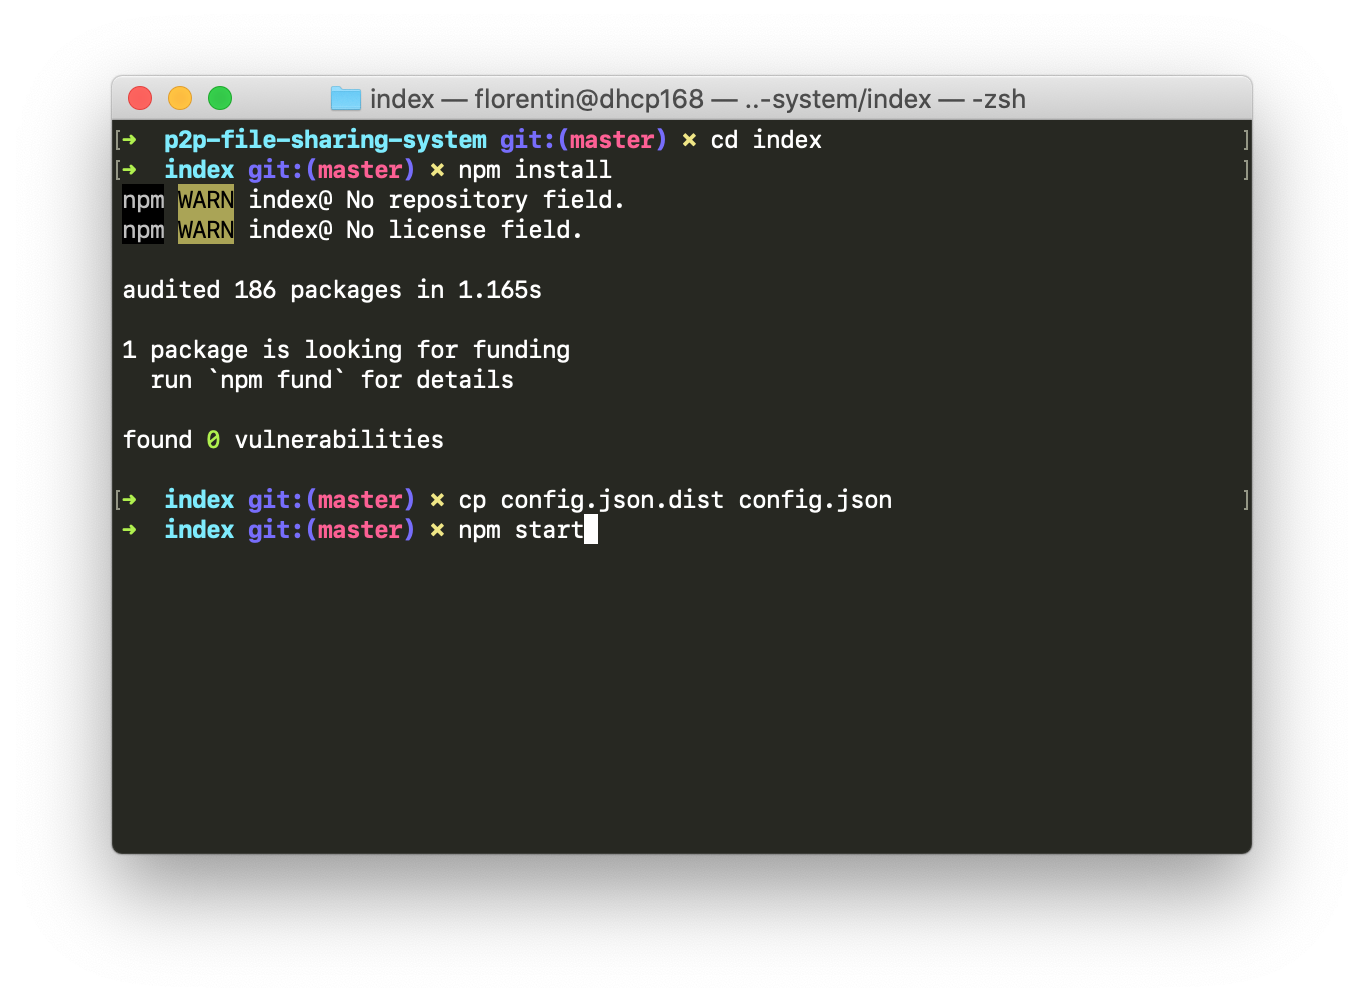
\includegraphics[width=0.7\linewidth]{assets/install-example.png}
	\caption{Example installation steps for Index}
	\label{fig:install-example}
\end{figure}

\noindent \textbf{Don't forget to follow this procedure for both softwares.}

\section{Usage}

\subsection{Index}

Once the \textbf{Index} software is configured and started, there is nothing more to do. Don't close the terminal window. You will be able to see the logs if you set \Verb+devMode+ to \Verb+true+ in \Verb+config.json+.

\noindent Press \Verb|cmd + C| to quit the software.

\subsection{Peer}

When you launch the \textbf{Peer} software, a CLI (command-line interface) will appear. You will be able to see the list of files shared or to download a file. Enter the command number to select your choice and press Enter to validate. Once an operation is finished, you will come back to the main menu.

\noindent If you get server errors when you start the software, make sure that the \textbf{Index} software is running and that you specified the right port in \Verb+config.json+.

\noindent Press \Verb|cmd + C| to quit the software.

\begin{figure}[h!]
	\centering
	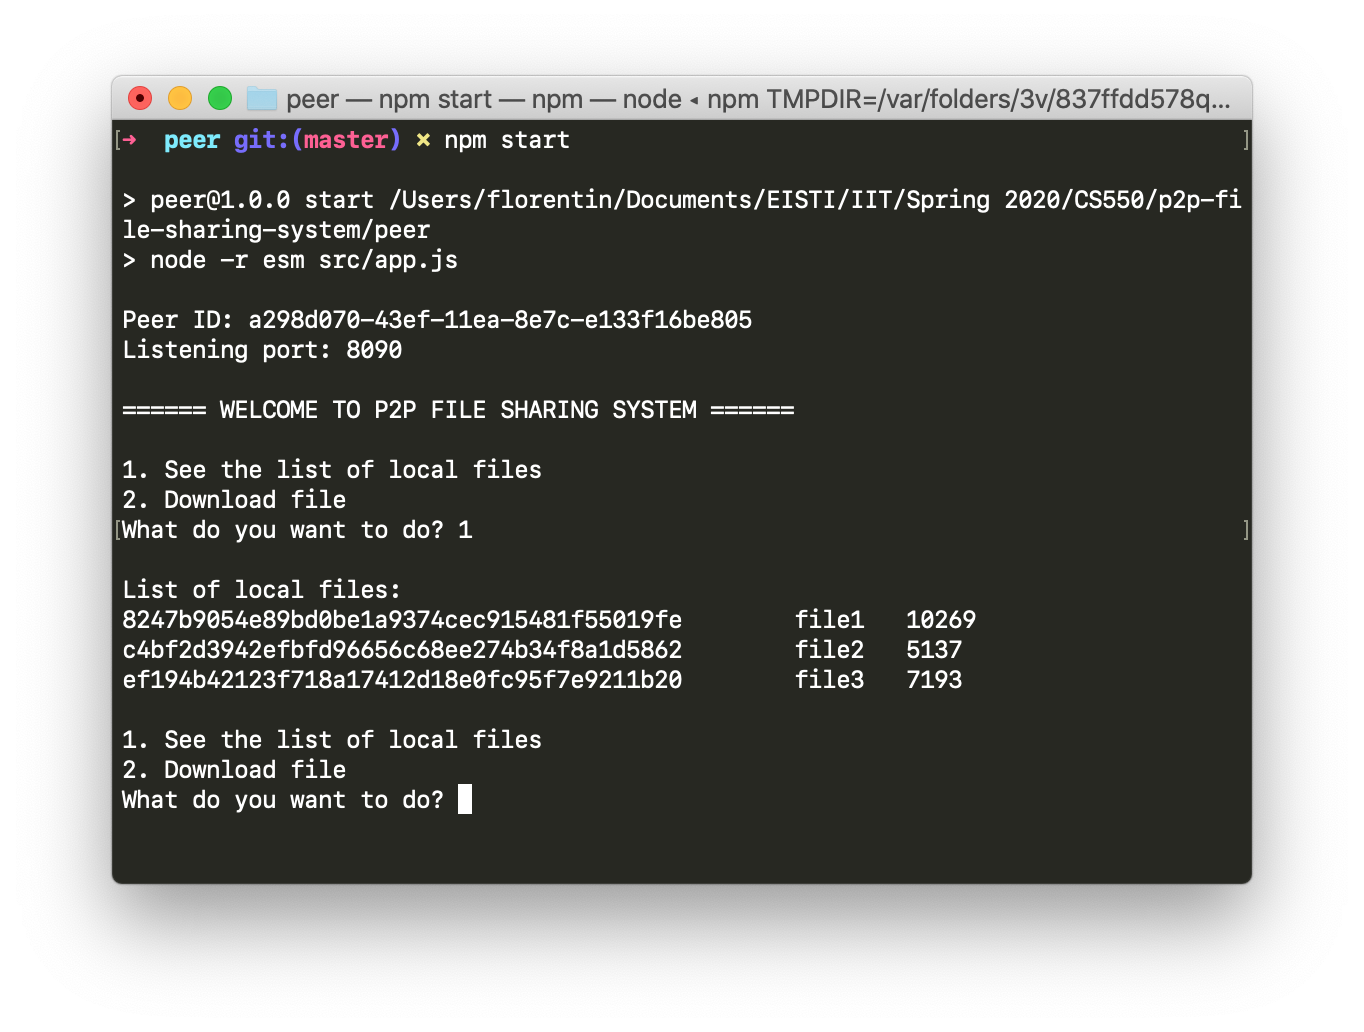
\includegraphics[width=0.7\linewidth]{assets/peer.png}
	\caption{Peer software}
	\label{fig:peer}
\end{figure}

\section{Test case}

% TODO: Add test case

\end{document}